\documentclass[9pt,twoside,lineno]{pnas-new}
% Use the lineno option to display guide line numbers if required.

\templatetype{pnassupportinginfo}

\title{Your main manuscript title}
\author{Author1, Author2 and Author3 (complete author list)}
\correspondingauthor{Corresponding Author name.\\E-mail: author.two@email.com}

\newcommand\mindate{25. Feb. 2020}
\newcommand\maxdate{31. Dec. 2020}
\newcommand\maxsamplingpercent{1}
\newcommand\gensimscalefactor{0.5}
\newcommand\travelcontextscalefactor{1}
\newcommand\outgroupisl{EPI\_ISL\_406798}
\newcommand\nswissseqs{X}
\newcommand\nsimseqs{Y}
\newcommand\ntravelseqs{Z}
\GISAIDpulldate{DD. Month 2021}

\newcommand\nchainsmin{296}
\newcommand\nchainsmax{1058}
\newcommand\minlargestchainsper{48}
\newcommand\maxlargestchainsper{27}
\newcommand\nspanningchainsmin{5}
\newcommand\nspanningchainsmax{1}

\newcommand\ncinongruentexposurechainsmax{7} 
\newcommand\nexposurechainsmax{106}
\newcommand\ncinongruentexposurechainsmin{14} 
\newcommand\nexposurechainsmin{64}
\newcommand\rankexpsamplemin{2}
\newcommand\rankexpsamplemax{1}

\begin{document}

%% Comment out or remove this line before generating final copy for submission; this will also remove the warning re: "Consecutive odd pages found".
\instructionspage  

\maketitle

%% Adds the main heading for the SI text. Comment out this line if you do not have any supporting information text.
\SItext


% \subsection*{Subhead}
% Type or paste text here. This should be additional explanatory text such as an extended technical description of results, full details of mathematical models, etc.   
\section{Sensitivity analyses}
We investigated the sensitivity of transmission chain summary statistics to different ratios of genetically similar foreign context sequences to focal Swiss sequences. Figure \ref{fig:sensitivity_context_set_size} shows that as the context set size is increased from a 1:1 to 3:1 ratio, the number of estimated transmission chains increases and the mean size of the transmission chains decreases. However, the greatest differences in estimated transmission chains result from the different assumptions about how to resolve phylogenetic uncertainty (smallest vs. largest plausible chains), not the size of the foreign context set. Therefore, we chose the 2:1 ratio as a balance of speed (smaller dataset = faster tree search convergence) and information content (larger dataset = more precise estimates of transmission chain import dates). We rely on the different polytomy resolutions from one such tree to incorporate most of the uncertainty in transmission chain definition.

\begin{figure*}[tbhp]
\centering
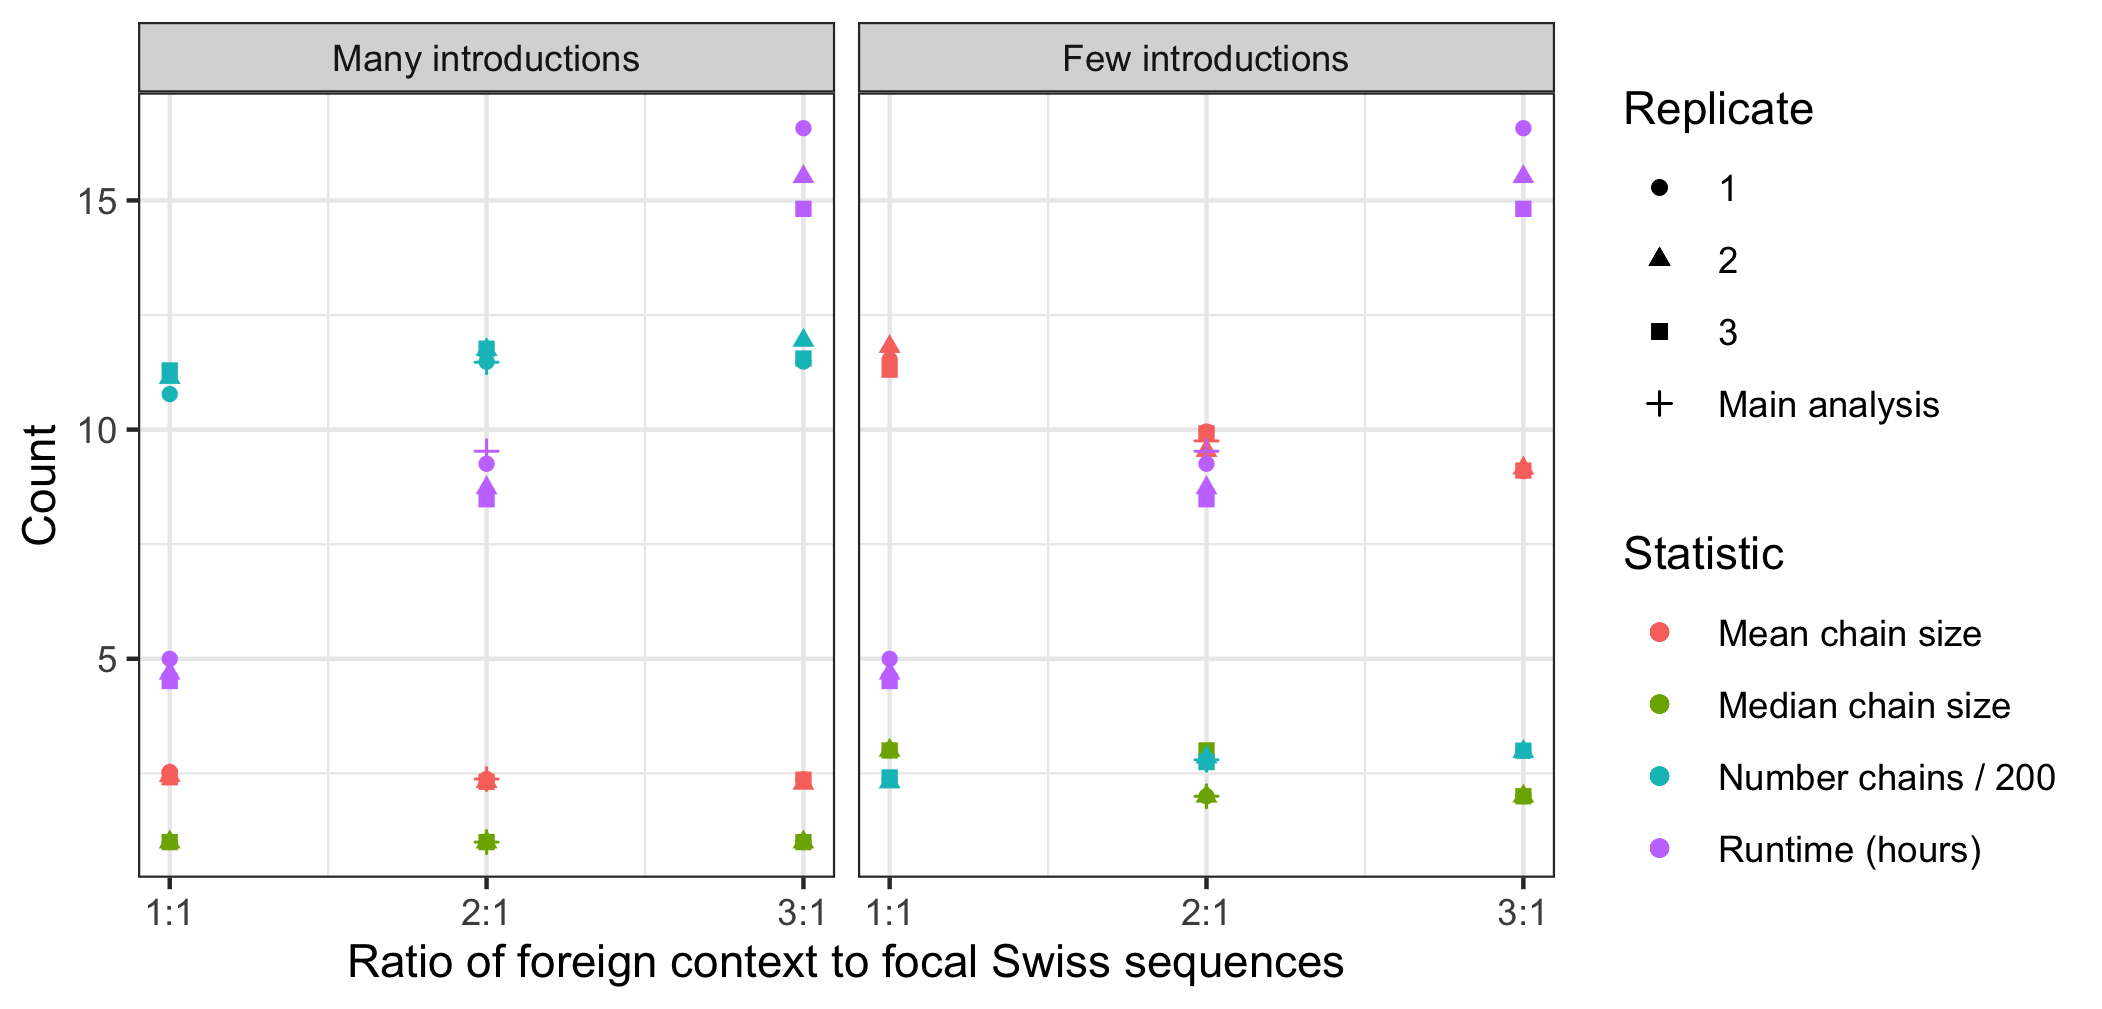
\includegraphics[width = 11.4cm]{figures/fig_SX_sensitivity_context_set_size.png}
\caption{Sensitivity of transmission chain summary statistics to different ratios of focal Swiss sequences to genetically similar foreign context sequences (1:1, 1:2, and 1:3).}  
\label{fig:sensitivity_context_set_size}
\end{figure*}

After deciding what size foreign context set to use, we investigated the sensitivity of transmission chain summary statistics to our heuristic definition of a transmission chain. Figure \ref{fig:sensitivity_m_p} shows that again, the greatest differences in estimated transmission chains result from different assumptions about how to resolve phylogenetic uncertainty, not the heuristic definition of a transmission chain. Therefore, we chose to define transmission chains based on maximum 3 exported lineages and maximum one consecutive export along a branch to allow for some exports but not arbitrarily many. 

\begin{figure*}[tbhp]
\centering
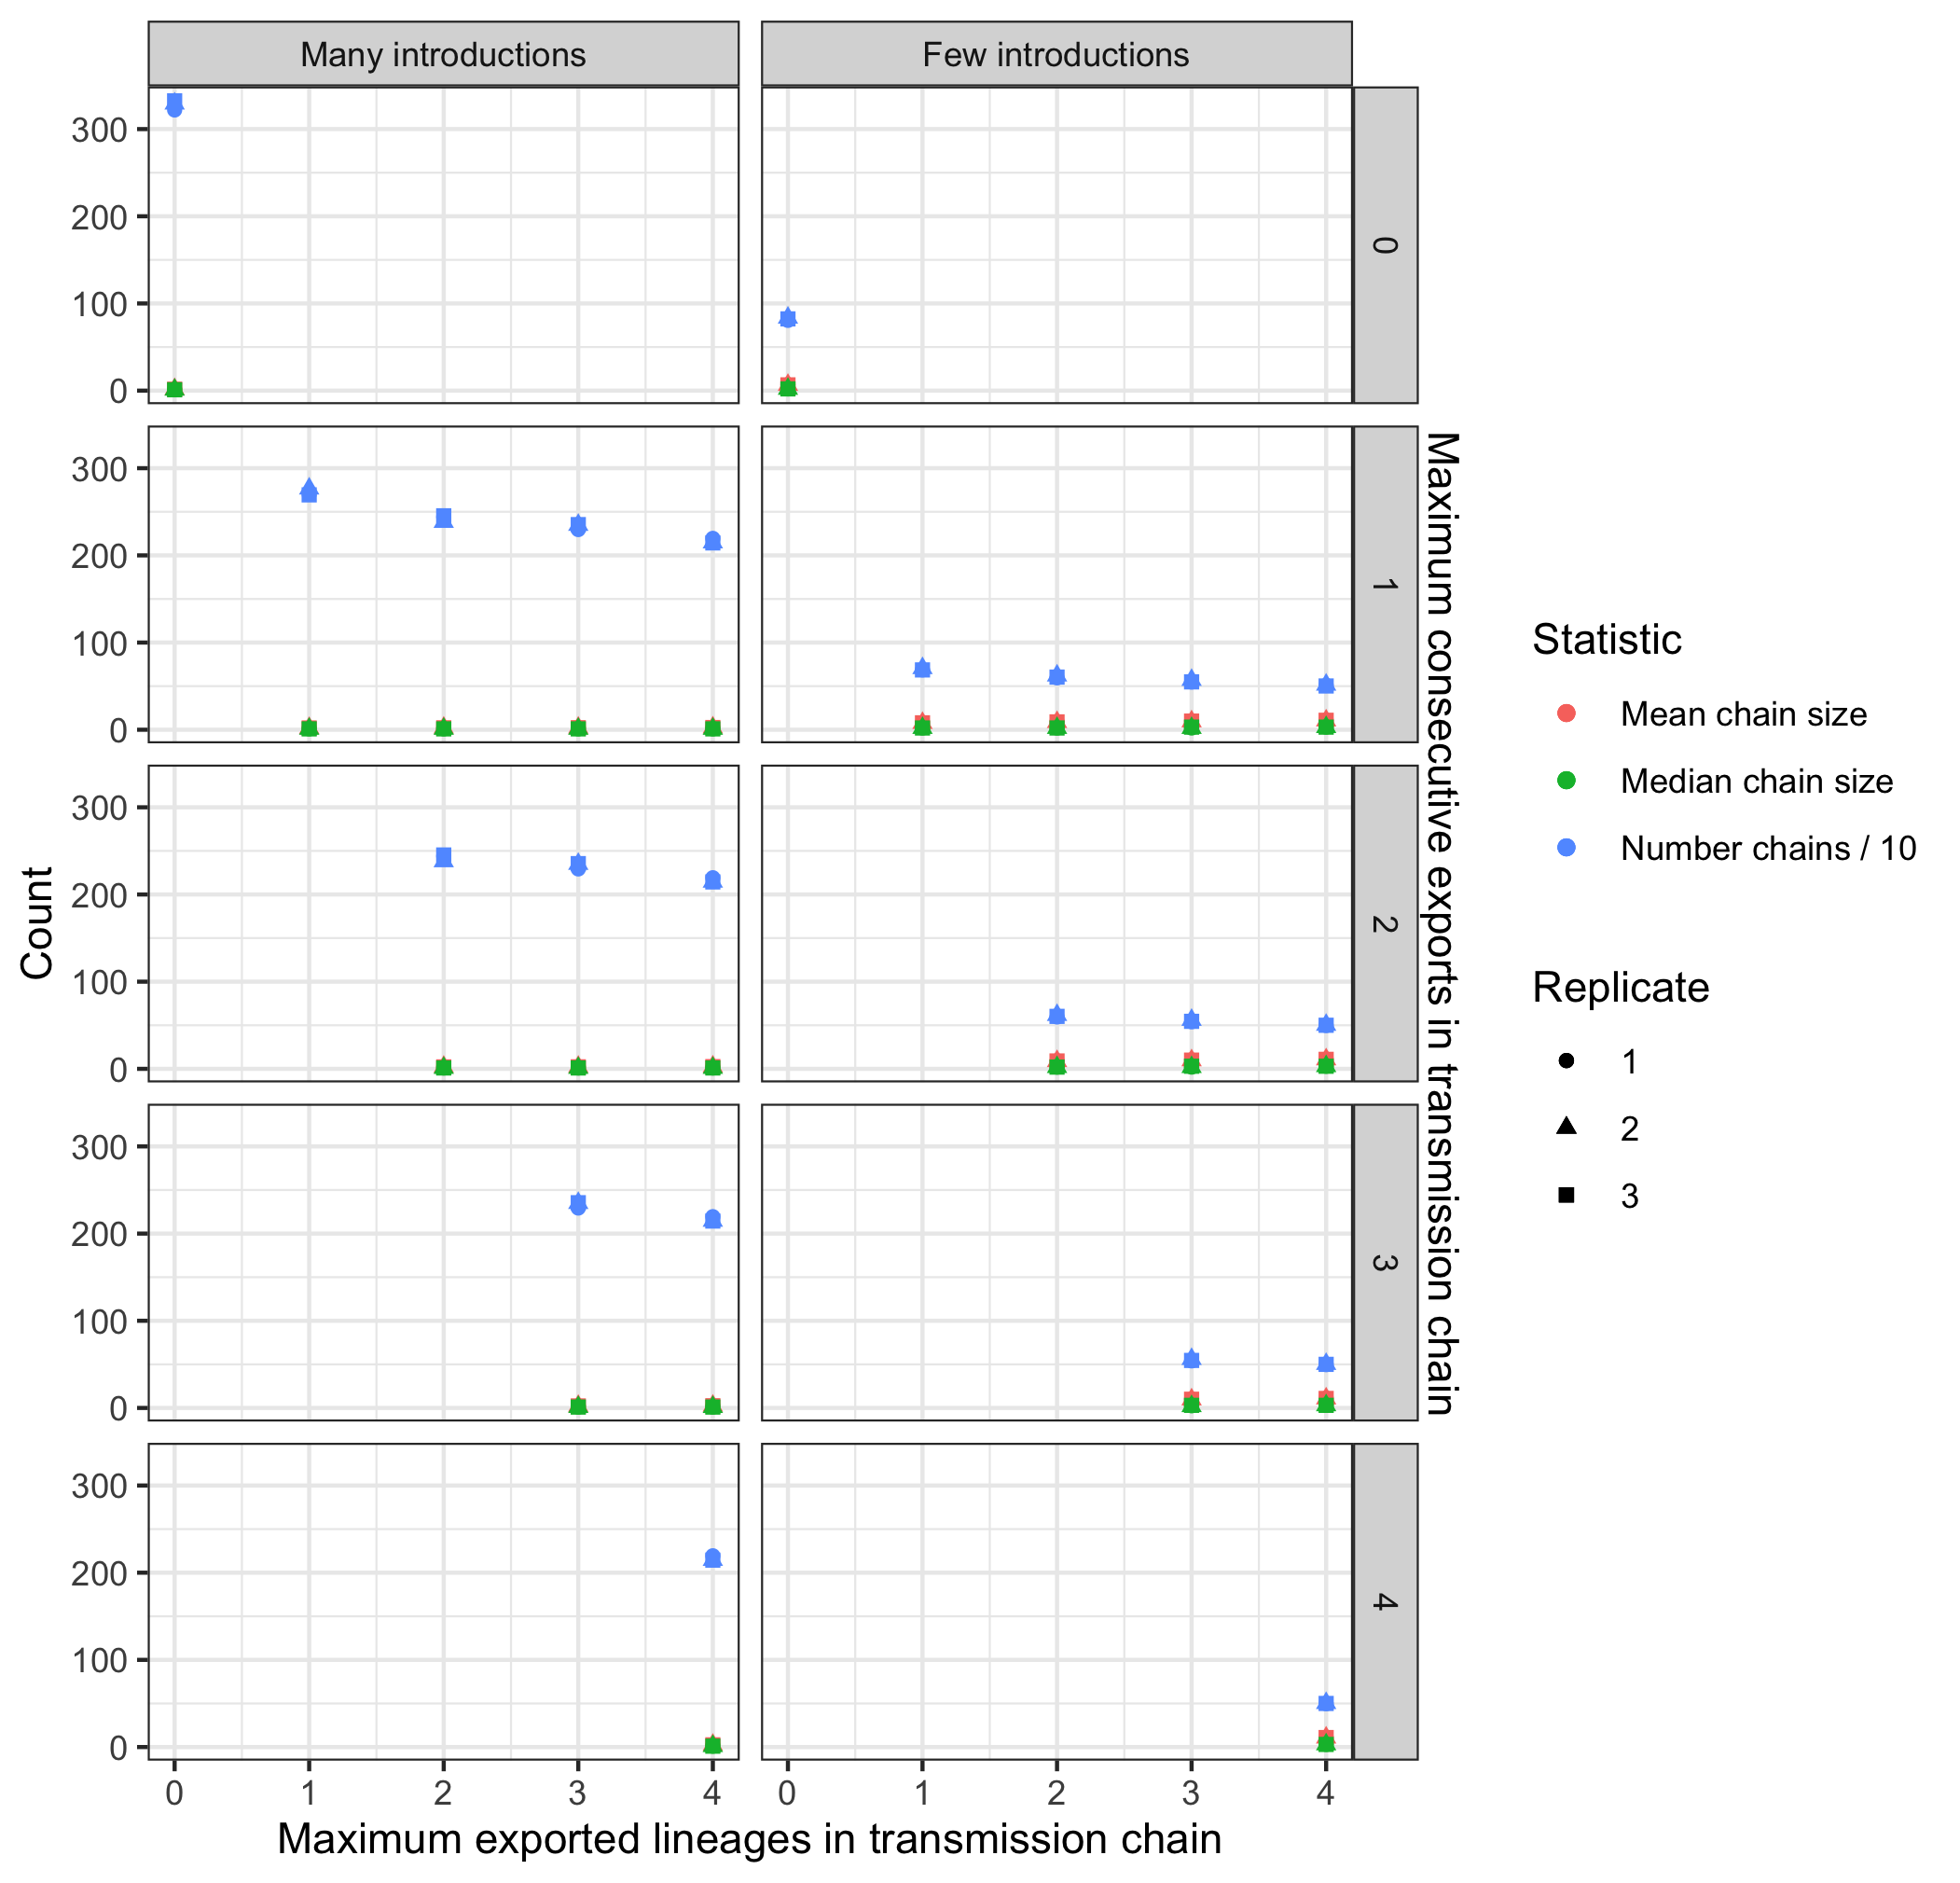
\includegraphics[width = 11.4cm]{figures/fig_SX_sensitivity_chain_defn.png}
\caption{Sensitivity of transmission chain summary statistics to different definitions of a transmission chain.}  
\label{fig:sensitivity_m_p}
\end{figure*}

Finally, we investigated the sensitivity of transmission chain summary statistics to the number of focal Swiss sequences analyzed.


\section*{Heading}
\subsection*{Subhead}
Type or paste text here. You may break this section up into subheads as needed (e.g., one section on ``Materials'' and one on ``Methods'').

\subsection*{Materials}
Add a materials subsection if you need to.

\subsection*{Methods}
Add a methods subsection if you need to.


%%% Each figure should be on its own page
\begin{figure}
\centering
\includegraphics[width=\textwidth]{example-image}
\caption{First figure}
\end{figure}

\begin{figure}
\centering
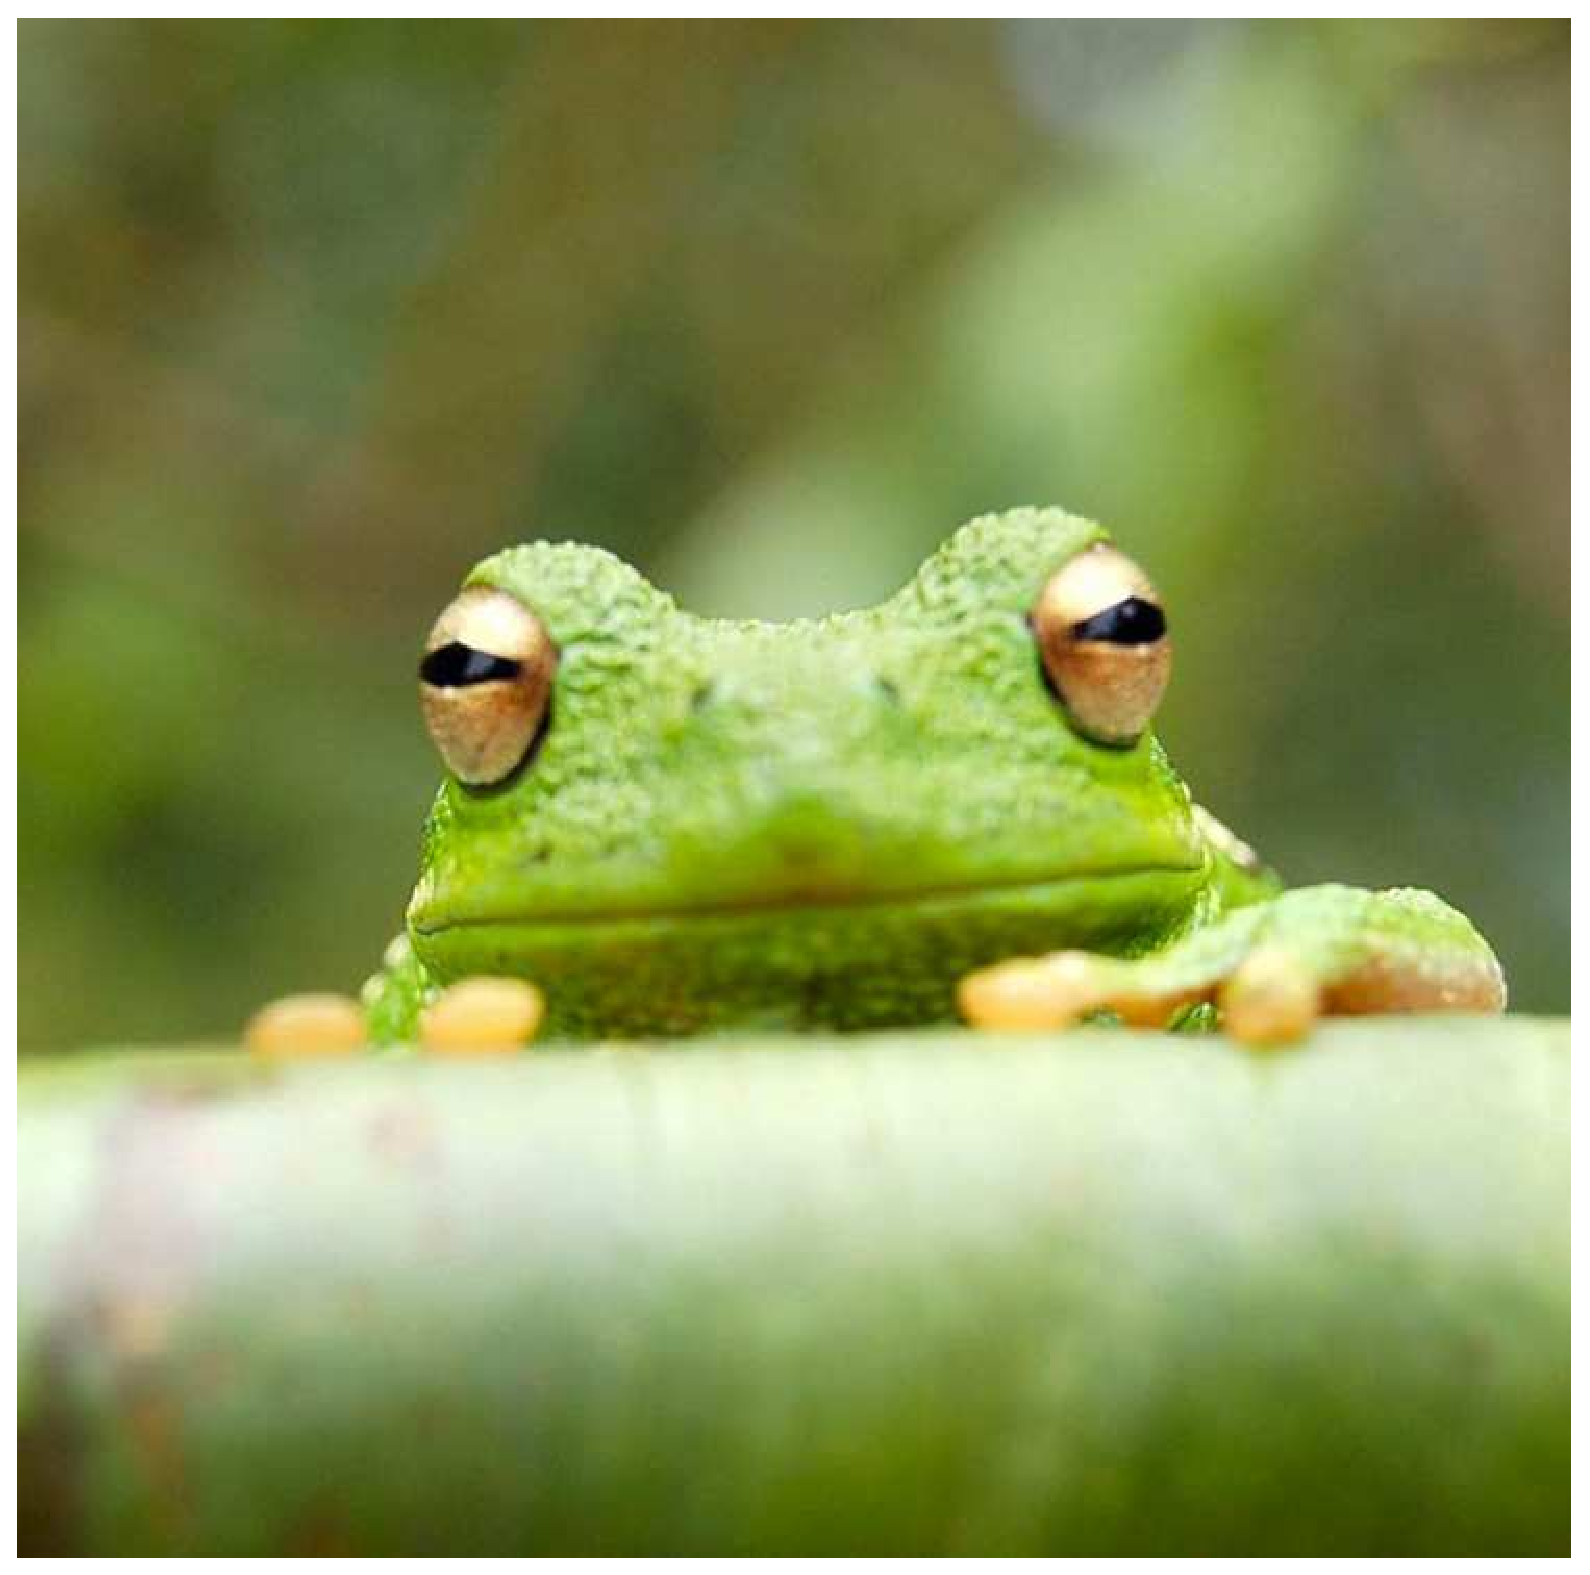
\includegraphics[width=\textwidth]{frog}
\caption{Second figure}
\end{figure}

\begin{table}\centering
\caption{This is a table}

\begin{tabular}{lrrr}
Species & CBS & CV & G3 \\
\midrule
1. Acetaldehyde & 0.0 & 0.0 & 0.0 \\
2. Vinyl alcohol & 9.1 & 9.6 & 13.5 \\
3. Hydroxyethylidene & 50.8 & 51.2 & 54.0\\
\bottomrule
\end{tabular}
\end{table}

%%% Add this line AFTER all your figures and tables
\FloatBarrier

\movie{Type legend for the movie here.}

\movie{Type legend for the other movie here. Adding longer text to show what happens, to decide on alignment and/or indentations.}

\movie{A third movie, just for kicks.}

\dataset{dataset_one.txt}{Type or paste legend here.}

\dataset{dataset_two.txt}{Type or paste legend here. Adding longer text to show what happens, to decide on alignment and/or indentations for multi-line or paragraph captions.}

\bibliography{pnas-sample}

\end{document}
